\documentclass[11pt,a4paper]{article}
\usepackage[utf8]{inputenc}
\usepackage[T1]{fontenc}
\usepackage[margin=0.95in]{geometry}
\usepackage{amsmath,amssymb}
\usepackage{tikz}
\usetikzlibrary{arrows.meta,positioning,decorations.pathreplacing}
\setlength{\parindent}{0pt}
\setlength{\parskip}{5pt}
\newcommand{\step}[1]{\textbf{Step #1.}}
\newcommand{\ub}{\bar u}
\tikzset{>=Stealth, box/.style={draw, rounded corners, minimum height=7mm, inner sep=4pt}}
\begin{document}

\begin{center}
{\Large\bfseries FK-LoRA, step by step}\\[3pt]
{\small Notes to the paper ``Never Forget What You Learn: FK-LoRA for Continual Learning Without Forgetting''}
\end{center}

%=====================================================================
\section*{1. The setting}

A frozen language model learns tasks $1, 2, \dots, T$ one after another. Each task gets its own
small adapter. An adapter is never changed after its task is learned.

\begin{center}
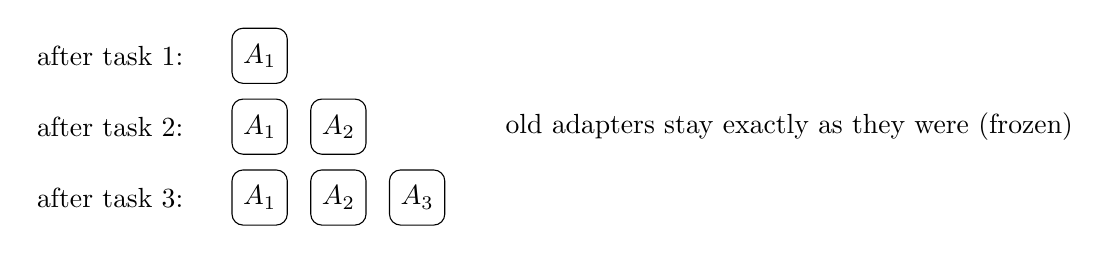
\begin{tikzpicture}
\node at (-1.3,0) {after task 1:}; \node[box] at (0.6,0) {$A_1$};
\node at (-1.3,-0.9) {after task 2:}; \node[box] at (0.6,-0.9) {$A_1$}; \node[box] at (1.6,-0.9) {$A_2$};
\node at (-1.3,-1.8) {after task 3:}; \node[box] at (0.6,-1.8) {$A_1$}; \node[box] at (1.6,-1.8) {$A_2$}; \node[box] at (2.6,-1.8) {$A_3$};
\node[right] at (3.6,-0.9) {old adapters stay exactly as they were (frozen)};
\end{tikzpicture}
\end{center}

A \emph{switch} looks at an input $x$ and picks one task. This choice is the \emph{route} $\rho_T(x)$
($T$ = number of tasks learned so far). If the route is $j$, the input is answered with adapters
$A_1,\dots,A_j$, that is, by the model as it was right after task $j$.

\begin{center}
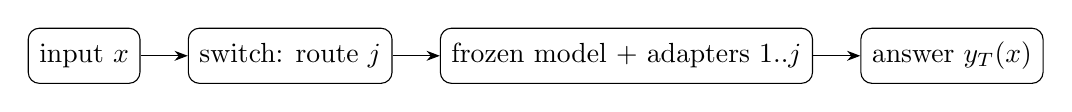
\begin{tikzpicture}
\node[box] (x) {input $x$};
\node[box, right=6mm of x] (s) {switch: route $j$};
\node[box, right=6mm of s] (m) {frozen model + adapters $1..j$};
\node[box, right=6mm of m] (y) {answer $y_T(x)$};
\draw[->] (x)--(s); \draw[->] (s)--(m); \draw[->] (m)--(y);
\end{tikzpicture}
\end{center}

%=====================================================================
\section*{2. An answer changes only if its route changes}

\step{1} Write the answer as a function. The model $F$ gets the input and the adapters $1..j$:
\[ y_T(x) = F(x;\ A_1,\dots,A_j), \qquad j=\rho_T(x). \]

\step{2} Take a later time $T' > T$ (more tasks have been learned). Suppose the route is the same:
\[ \rho_{T'}(x) = \rho_T(x) = j. \]

\step{3} Then the answer at $T'$ uses the same list of adapters:
\[ y_{T'}(x) = F(x;\ A_1,\dots,A_j). \]

\step{4} $A_1,\dots,A_j$ are frozen, so they are the same objects at $T$ and at $T'$. $F$ is the same
frozen model and it has no randomness. Same function, same inputs $\Rightarrow$ same output:
\[ \boxed{\ \rho_{T'}(x) = \rho_T(x) \ \Longrightarrow\ y_{T'}(x) = y_T(x)\ } \]

\begin{center}
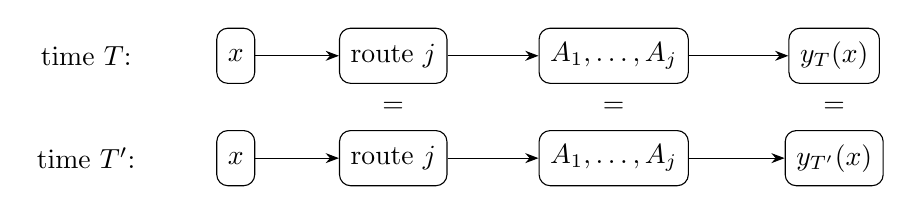
\begin{tikzpicture}
\node at (-1.5,0) {time $T$:}; \node[box] (a1) at (0.4,0) {$x$}; \node[box] (a2) at (2.4,0) {route $j$}; \node[box] (a3) at (5.2,0) {$A_1,\dots,A_j$}; \node[box] (a4) at (8.0,0) {$y_T(x)$};
\node at (-1.5,-1.3) {time $T'$:}; \node[box] (b1) at (0.4,-1.3) {$x$}; \node[box] (b2) at (2.4,-1.3) {route $j$}; \node[box] (b3) at (5.2,-1.3) {$A_1,\dots,A_j$}; \node[box] (b4) at (8.0,-1.3) {$y_{T'}(x)$};
\draw[->] (a1)--(a2); \draw[->] (a2)--(a3); \draw[->] (a3)--(a4); \draw[->] (b1)--(b2); \draw[->] (b2)--(b3); \draw[->] (b3)--(b4);
\node at (2.4,-0.65) {$=$}; \node at (5.2,-0.65) {$=$}; \node at (8.0,-0.65) {$=$};
\end{tikzpicture}
\end{center}

\textbf{Meaning.} Forgetting can only come from a changed route. So we only have to study the rule
that sets the route. The paper has three rules: FinderLoRA, KeeperLoRA and ClaimLoRA.

%=====================================================================
\section*{3. FinderLoRA: find the task without an instruction}

\subsection*{3.1 The feature}

\step{1} Give the text $x$ to the frozen model (no adapter). It returns one vector per token:
$h_1, h_2, \dots, h_n$, each in $\mathbb{R}^d$.

\step{2} Average them. This is the feature of the input:
\[ u(x) = \frac{1}{n}\,(h_1 + h_2 + \dots + h_n) \in \mathbb{R}^d . \]

\step{3} Put a $1$ at the end (this gives the rule a constant term):
\[ \ub(x) = (u(x),\, 1) \in \mathbb{R}^{d+1}. \]

\begin{center}
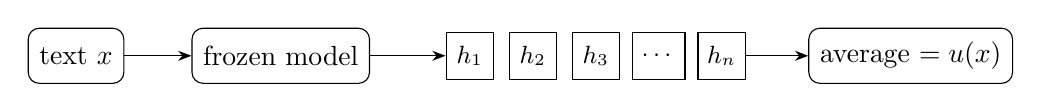
\begin{tikzpicture}
\node[box] (t) at (0,0) {text $x$};
\node[box] (e) at (2.6,0) {frozen model};
\foreach \i/\l in {0/$h_1$,1/$h_2$,2/$h_3$,3/$\cdots$,4/$h_n$} { \node[draw, minimum size=6mm] (h\i) at (5.0+\i*0.8,0) {\small \l}; }
\node[box] (u) at (10.6,0) {average $=u(x)$};
\draw[->] (t)--(e); \draw[->] (e)--(h0); \draw[->] (h4)--(u);
\end{tikzpicture}
\end{center}

\subsection*{3.2 What we want from the rule}

\step{4} For every task $c$ we want a weight vector $w_c \in \mathbb{R}^{d+1}$ and a score
\[ \text{score}_c(x) = \ub(x)^{\top} w_c . \]

\step{5} The score of task $c$ should be near $1$ on inputs of task $c$ and near $0$ on inputs of the
other tasks. Write this target as $t$:
\[ t = 1 \ \text{ if } x \text{ belongs to task } c, \qquad t = 0 \ \text{ otherwise.} \]

\begin{center}
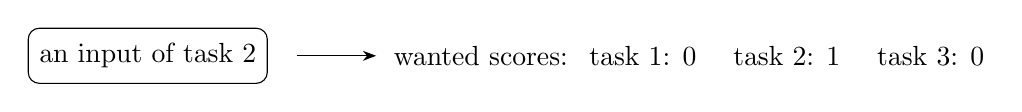
\begin{tikzpicture}
\node[box] at (0,0) {an input of task 2};
\draw[->] (1.9,0)--(2.9,0);
\node[right] at (3.0,0) {wanted scores: \ task 1: $0$ \quad task 2: $1$ \quad task 3: $0$};
\end{tikzpicture}
\end{center}

\subsection*{3.3 The error, for one task $c$}

\step{6} The error on one input is the squared difference between score and target:
\[ \bigl(\ub(x)^{\top} w_c - t\bigr)^2 . \]

\step{7} Average it over the inputs of each task $k$, add up over the tasks, and add a small penalty
$\varepsilon\,w_c^{\top}w_c$ that keeps the weights small:
\[ L(w_c) \;=\; \sum_{k=1}^{T}\ \underset{x \in \text{task } k}{\text{mean}} \bigl(\ub(x)^{\top} w_c - t\bigr)^2 \;+\; \varepsilon\, w_c^{\top} w_c . \]

\subsection*{3.4 The derivative, piece by piece}

\step{8} One squared term. Call the inside $a = \ub^{\top}w_c - t$. The chain rule gives
\[ \frac{\partial}{\partial w_c}\, a^2 \;=\; 2a\,\frac{\partial a}{\partial w_c} \;=\; 2\,(\ub^{\top}w_c - t)\,\ub . \]
(Because $a$ is linear in $w_c$, its derivative is just $\ub$.)

\step{9} Write the same thing with the vector first: $\ 2\,\ub\,(\ub^{\top}w_c - t) \;=\; 2\,\ub\,\ub^{\top} w_c \;-\; 2\,t\,\ub .$

\step{10} The penalty: $\ \dfrac{\partial}{\partial w_c}\ \varepsilon\,w_c^{\top}w_c = 2\,\varepsilon\,w_c .$

\step{11} Put Steps 9 and 10 into $L$ (the mean and the sum just stay in front):
\[ \frac{\partial L}{\partial w_c} \;=\; 2\sum_{k}\ \text{mean}\ \ub\,\ub^{\top}\, w_c \;-\; 2\sum_{k}\ \text{mean}\ t\,\ub \;+\; 2\,\varepsilon\, w_c . \]

\subsection*{3.5 Simplify the two sums}

\step{12} First sum. Name the average of $\ub\,\ub^{\top}$ over the inputs of task $k$:
\[ G_k \;=\; \underset{x \in \text{task } k}{\text{mean}}\ \ub(x)\,\ub(x)^{\top} \qquad \text{(a matrix)}. \]
So the first sum is $\ \bigl(\sum_k G_k\bigr)\, w_c$.

\step{13} Second sum. $t = 0$ for every task except task $c$, where $t=1$. So only task $c$ is left:
\[ \sum_{k}\ \text{mean}\ t\,\ub \;=\; \underset{x \in \text{task } c}{\text{mean}}\ \ub(x) \;=:\; v_c \qquad \text{(a vector)}. \]

\step{14} The derivative is now short:
\[ \frac{\partial L}{\partial w_c} \;=\; 2\Bigl(\sum_k G_k\Bigr) w_c \;-\; 2\,v_c \;+\; 2\,\varepsilon\,w_c . \]

\subsection*{3.6 Solve}

\step{15} At the minimum the derivative is zero. Divide by 2 and move $v_c$ to the right:
\[ \Bigl(\sum_k G_k\Bigr) w_c + \varepsilon\,w_c = v_c
   \quad\Longrightarrow\quad \Bigl(\sum_k G_k + \varepsilon I\Bigr)\, w_c = v_c . \]

\step{16} Multiply both sides by the inverse matrix. (It exists: every $G_k$ is positive
semi-definite and $\varepsilon I$ makes the sum positive definite.)
\[ w_c \;=\; \Bigl(\sum_k G_k + \varepsilon I\Bigr)^{-1} v_c . \]

\step{17} The matrix in front is the same for every task $c$. Put the vectors $w_1,\dots,w_T$ side
by side as the columns of one matrix $V_T$:
\[ \boxed{\ V_T = \Bigl(\sum_{k \le T} G_k + \varepsilon I\Bigr)^{-1} [\,v_1,\dots,v_T\,]\ } \]

\step{18} The route is the task with the largest score:
\[ \boxed{\ \rho_T(x) = \arg\max_{k \le T}\ \bigl(\ub(x)^{\top} V_T\bigr)_k\ } \]

\begin{center}
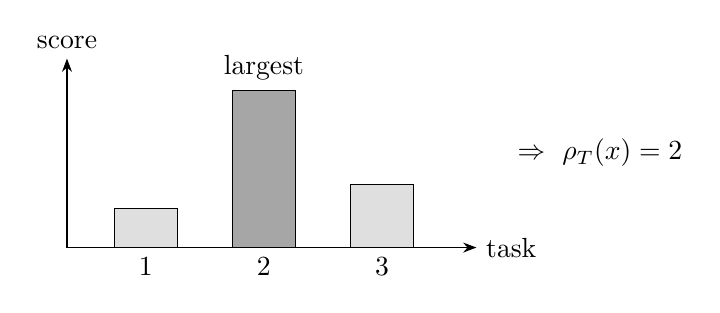
\begin{tikzpicture}
\draw[->] (0,0)--(5.2,0) node[right]{task};
\draw[->] (0,0)--(0,2.4) node[above]{score};
\draw[fill=gray!25] (0.6,0) rectangle (1.4,0.5);
\draw[fill=gray!70] (2.1,0) rectangle (2.9,2.0);
\draw[fill=gray!25] (3.6,0) rectangle (4.4,0.8);
\node[below] at (1.0,0) {1}; \node[below] at (2.5,0) {2}; \node[below] at (4.0,0) {3};
\node[above] at (2.5,2.0) {largest};
\node[right] at (5.6,1.2) {$\Rightarrow\ \rho_T(x) = 2$};
\end{tikzpicture}
\end{center}

\subsection*{3.7 A check in one dimension}

Take $d=1$, no constant, two tasks. Then $G_k$ is the number $g_k = \text{mean}\ u^2$ and $v_c$ is the
number $\text{mean}\ u$ of task $c$. Step 16 becomes
\[ w_c = \frac{v_c}{g_1 + g_2 + \varepsilon} . \]
A task whose inputs have a larger average $u$ gets a larger weight, as it should.

\subsection*{3.8 What happens when a new task arrives}

Only two things are stored: the sum $S=\sum_k G_k$ and the list of vectors $v_k$.
A new task adds its $G_{T+1}$ to $S$ and appends its $v_{T+1}$. Nothing else is touched.

\begin{center}
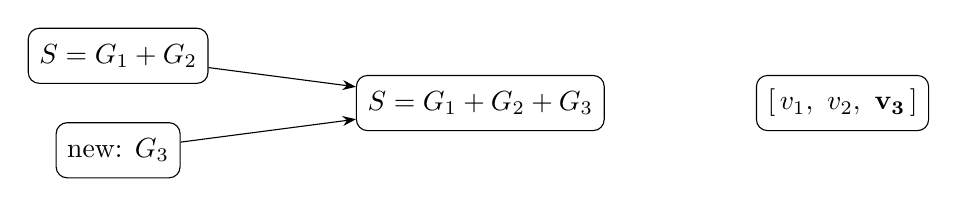
\begin{tikzpicture}
\node[box] (S) at (0,0) {$S = G_1 + G_2$};
\node[box] (g) at (0,-1.2) {new: $G_3$};
\node[box] (S2) at (4.6,-0.6) {$S = G_1 + G_2 + G_3$};
\draw[->] (S)--(S2); \draw[->] (g)--(S2);
\node[box] (v) at (9.2,-0.6) {$[\,v_1,\ v_2,\ \mathbf{v_3}\,]$};
\end{tikzpicture}
\end{center}

A sum does not depend on the order in which it was added. So $V_T$ is the same for every order of
the tasks, no old input has to be stored, and every task has its own column: no task is blocked.

%=====================================================================
\section*{4. The audit: how many answers changed?}

\subsection*{4.1 Set some inputs aside}

\step{1} When task $j$ arrives, split its inputs: most are used to build $G_j$ and $v_j$ (\emph{fit}),
and $m$ are kept aside (\emph{held-out}). The rule never uses the held-out inputs.

\begin{center}
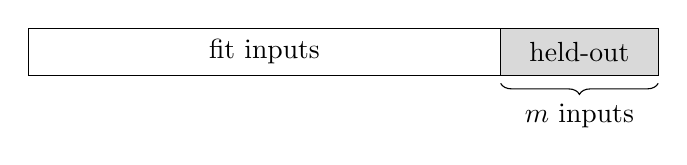
\begin{tikzpicture}
\draw (0,0) rectangle (6.0,0.6); \draw[fill=gray!30] (6.0,0) rectangle (8.0,0.6);
\node at (3.0,0.3) {fit inputs}; \node at (7.0,0.3) {held-out};
\draw[decorate, decoration={brace, mirror, amplitude=4pt}] (6.0,-0.1)--(8.0,-0.1) node[midway, below=4pt]{$m$ inputs};
\end{tikzpicture}
\end{center}

\step{2} Fix two times $T < T'$. For held-out input number $i$ write
\[ I_i = 1 \ \text{ if its route at } T' \text{ differs from its route at } T, \qquad I_i = 0 \ \text{ otherwise.} \]

\step{3} Count them: \quad $H = I_1 + I_2 + \dots + I_m$.

\begin{center}
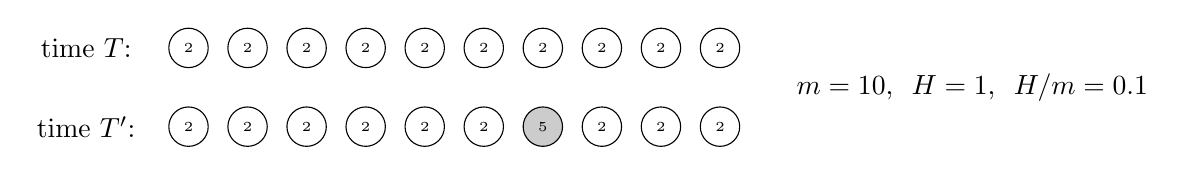
\begin{tikzpicture}
\node at (-1.3,0.5) {time $T$:}; \node at (-1.3,-0.5) {time $T'$:};
\foreach \i in {0,...,9} { \node[draw, circle, minimum size=5mm, inner sep=0pt] at (\i*0.75,0.5) {\tiny 2}; }
\foreach \i in {0,1,2,3,4,5,7,8,9} { \node[draw, circle, minimum size=5mm, inner sep=0pt] at (\i*0.75,-0.5) {\tiny 2}; }
\node[draw, circle, fill=gray!40, minimum size=5mm, inner sep=0pt] at (6*0.75,-0.5) {\tiny 5};
\node[right] at (7.6,0) {$m=10$, \ $H=1$, \ $H/m = 0.1$};
\end{tikzpicture}

{\small Ten held-out inputs of task 2. The number in a circle is the route. One input moved to task 5.}
\end{center}

\subsection*{4.2 Why $H/m$ is the right estimate}

\step{4} Let $X$ be a \emph{new} input of task $j$, and let $p$ be the chance that its route changes:
\[ p = \Pr[\rho_{T'}(X) \neq \rho_T(X)]. \]

\step{5} A held-out input is drawn in the same way as $X$, and the rule was built without it. So each
$I_i$ is $1$ with the same chance $p$: \quad $\mathbb{E}[I_i] = p$.

\step{6} The expected value of a sum is the sum of the expected values:
\[ \mathbb{E}[H] = \mathbb{E}[I_1] + \dots + \mathbb{E}[I_m] = m\,p
   \quad\Longrightarrow\quad \mathbb{E}\!\left[\frac{H}{m}\right] = p . \]

\step{7} From Section 2: if the answer changed, the route changed. So the event ``answer changed'' is
inside the event ``route changed'', and a smaller event has a smaller chance:
\[ \boxed{\ \Pr[\text{answer changed}] \;\le\; \Pr[\text{route changed}] \;=\; p \;=\; \mathbb{E}\!\left[\frac{H}{m}\right]\ } \]

\subsection*{4.3 An upper limit, with an example}

\step{8} If the held-out inputs are independent, $H$ is a count of $m$ yes/no trials with chance $p$
(binomial). Take the case $H = 0$ (no held-out input changed). The chance of seeing this is
\[ \Pr[H=0] = (1-p)^m . \]

\step{9} We only keep values of $p$ for which this is not too unlikely, say at least $5\%$:
\[ (1-p)^m \ge 0.05 \ \Longrightarrow\ 1-p \ge 0.05^{1/m} \ \Longrightarrow\ p \le 1 - 0.05^{1/m} . \]

\step{10} With $m = 200$: \quad $p \le 1 - 0.05^{1/200} = 0.0149$, about $1.5\%$.

So ``no change among 200 held-out inputs'' means: at most about $1.5\%$ of the answers of this task
changed (with $95\%$ confidence). For $H > 0$ the same idea gives a larger limit. The limit holds for
one task and one pair of times.

%=====================================================================
\section*{5. KeeperLoRA: an older task keeps what it found}

\subsection*{5.1 The rule}

\step{1} \textbf{Margin.} A new task $k$ arrives. On an input $x$, compare its score with the best
older score:
\[ \xi_k(x) \;=\; \text{score}_k(x) \;-\; \max_{i<k}\ \text{score}_i(x). \]
$\xi_k(x) > 0$ means: the newcomer is ahead on $x$.

\begin{center}
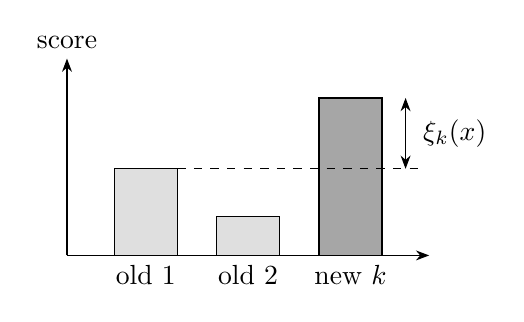
\begin{tikzpicture}
\draw[->] (0,0)--(4.6,0); \draw[->] (0,0)--(0,2.5) node[above]{score};
\draw[fill=gray!25] (0.6,0) rectangle (1.4,1.1); \draw[fill=gray!25] (1.9,0) rectangle (2.7,0.5); \draw[fill=gray!70] (3.2,0) rectangle (4.0,2.0);
\node[below] at (1.0,0) {old 1}; \node[below] at (2.3,0) {old 2}; \node[below] at (3.6,0) {new $k$};
\draw[dashed] (1.4,1.1)--(4.5,1.1);
\draw[<->] (4.3,1.1)--(4.3,2.0); \node[right] at (4.4,1.55) {$\xi_k(x)$};
\end{tikzpicture}
\end{center}

\step{2} \textbf{Threshold.} Take an older task $j$ and its $m$ held-out inputs. Compute the margin
$\xi_k$ of each and sort them. Pick the $(\nu+1)$-th largest (with $\nu=2$: the third largest).
Do this for every older task. The threshold $\eta_k$ is the largest of these numbers, and it is
never below $0$.

\begin{center}
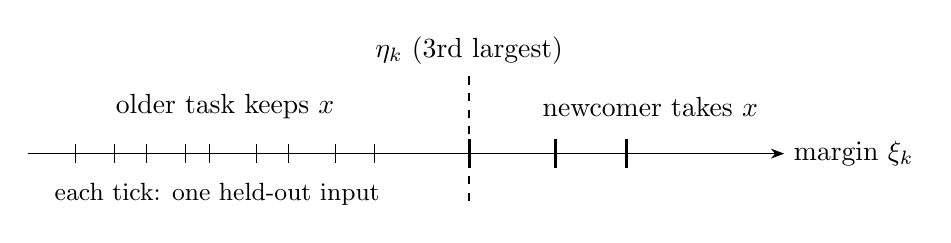
\begin{tikzpicture}
\draw[->] (0,0)--(9.6,0) node[right]{margin $\xi_k$};
\foreach \p in {0.6,1.1,1.5,2.0,2.3,2.9,3.3,3.9,4.4} { \draw (\p,-0.12)--(\p,0.12); }
\foreach \p in {5.6,6.7,7.6} { \draw[very thick] (\p,-0.18)--(\p,0.18); }
\draw[dashed, thick] (5.6,-0.6)--(5.6,1.0) node[above]{$\eta_k$ (3rd largest)};
\node at (2.5,0.6) {older task keeps $x$};
\node at (7.9,0.6) {newcomer takes $x$};
\node[below] at (2.4,-0.25) {\small each tick: one held-out input};
\end{tikzpicture}
\end{center}

\step{3} \textbf{Rule.} The newcomer $k$ takes $x$ only if $\xi_k(x) > \eta_k$. The route of $x$ is the
newest task that took it.

\subsection*{5.2 How often can one newcomer take an input of task $j$?}

\step{4} Let $X$ be a new input of task $j$. Put its margin next to the margins of the $m$ held-out
inputs. That makes $m+1$ numbers, all drawn in the same way.

\step{5} Sort the $m+1$ numbers from largest to smallest. Because they are drawn in the same way,
$X$ is equally likely to land in each of the $m+1$ places:
\[ \Pr[X \text{ is in place } r] = \frac{1}{m+1} \quad \text{for } r = 1,\dots,m+1 . \]

\step{6} Suppose the newcomer takes $X$: $\ \xi_k(X) > \eta_k$. By Step 2, $\eta_k$ is at least the
$(\nu+1)$-th largest held-out margin. So at most $\nu$ held-out margins are above $\xi_k(X)$. So $X$ is
in one of the first $\nu+1$ places.

\begin{center}
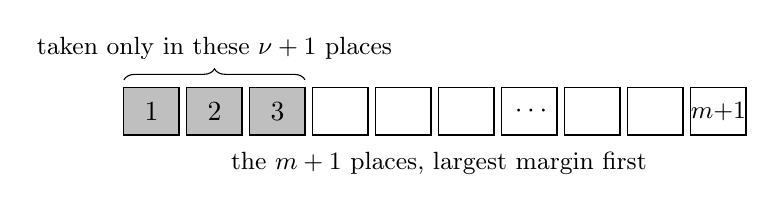
\begin{tikzpicture}
\foreach \i in {0,1,2} { \draw[fill=gray!50] (\i*0.8,0) rectangle (\i*0.8+0.7,0.6); }
\foreach \i in {3,...,9} { \draw (\i*0.8,0) rectangle (\i*0.8+0.7,0.6); }
\node at (0.35,0.3) {1}; \node at (1.15,0.3) {2}; \node at (1.95,0.3) {3}; \node at (5.2,0.3) {$\cdots$}; \node at (7.55,0.3) {\small $m{+}1$};
\draw[decorate, decoration={brace, amplitude=4pt}] (0,0.7)--(2.3,0.7) node[midway, above=4pt]{\small taken only in these $\nu+1$ places};
\node[below] at (4.0,-0.1) {\small the $m+1$ places, largest margin first};
\end{tikzpicture}
\end{center}

\step{7} Add the chances of these $\nu+1$ places (Step 5):
\[ \Pr[\text{newcomer } k \text{ takes } X] \;\le\; \underbrace{\frac{1}{m+1} + \dots + \frac{1}{m+1}}_{\nu+1 \text{ times}} \;=\; \frac{\nu+1}{m+1}. \]

\subsection*{5.3 All later tasks together}

\step{8} The route of $X$ changes at the arrival of task $k$ only if task $k$ takes $X$. Later tasks
are $k = j+1,\ j+2,\ \dots,\ T_{\text{end}}$. That is $T_{\text{end}} - j$ tasks.

\step{9} The chance that \emph{at least one} of several events happens is at most the sum of their
chances:
\[ \Pr[\text{some later task takes } X] \;\le\; \sum_{k=j+1}^{T_{\text{end}}} \frac{\nu+1}{m+1} . \]

\step{10} All terms of the sum are equal, and there are $T_{\text{end}}-j$ of them:
\[ \boxed{\ \Pr[\text{the route of } X \text{ ever changes}] \;\le\; \frac{(T_{\text{end}}-j)\,(\nu+1)}{m+1}\ } \]

\begin{center}
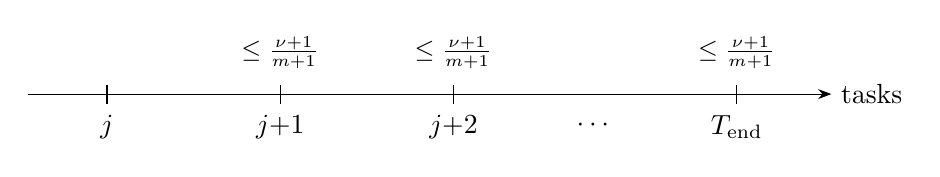
\begin{tikzpicture}
\draw[->] (0,0)--(10.2,0) node[right]{tasks};
\foreach \p/\l in {1/$j$,3.2/$j{+}1$,5.4/$j{+}2$,9.0/$T_{\text{end}}$} { \draw (\p,-0.12)--(\p,0.12); \node[below] at (\p,-0.15) {\l}; }
\node at (7.2,-0.4) {$\cdots$};
\foreach \p in {3.2,5.4,9.0} { \node[above] at (\p,0.2) {\small $\le \frac{\nu+1}{m+1}$}; }
\end{tikzpicture}
\end{center}

\step{11} \textbf{Example.} $m = 200$, $\nu = 2$, four later tasks:
$\ \dfrac{4 \cdot 3}{201} = 0.06$, so at most $6\%$.

This number is known \emph{before} any later task arrives. It is a loose bound, and it needs that the
later tasks are fixed without looking at $X$ or at the held-out inputs.

%=====================================================================
\section*{6. ClaimLoRA: zones, when inputs carry an instruction}

\subsection*{6.1 From an input to one vector}

\step{1} An input of task $k$ is the task's instruction followed by the example. The instruction is
the same for every input of the task. Its length is $n_k$ tokens.

\begin{center}
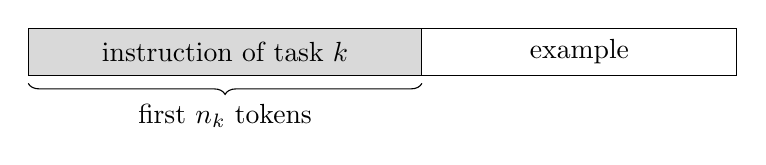
\begin{tikzpicture}
\draw[fill=gray!30] (0,0) rectangle (5.0,0.6); \draw (5.0,0) rectangle (9.0,0.6);
\node at (2.5,0.3) {instruction of task $k$}; \node at (7.0,0.3) {example};
\draw[decorate, decoration={brace, mirror, amplitude=4pt}] (0,-0.1)--(5.0,-0.1) node[midway, below=4pt]{first $n_k$ tokens};
\end{tikzpicture}
\end{center}

\step{2} Every token $x_i$ has a frozen word-vector $E_{x_i}$ and a weight $w(x_i)$ (rare words weigh
more). Take the weighted average of the first $n$ tokens:
\[ \varphi_n(x) = \frac{w(x_1)E_{x_1} + \dots + w(x_n)E_{x_n}}{w(x_1) + \dots + w(x_n)} . \]

\begin{center}
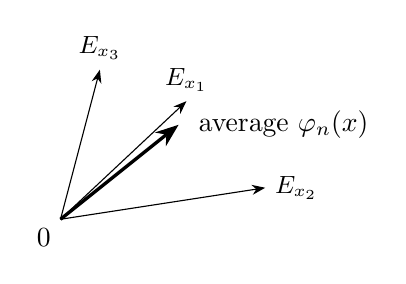
\begin{tikzpicture}
\draw[->] (0,0)--(1.6,1.5) node[above]{\small $E_{x_1}$};
\draw[->] (0,0)--(2.6,0.4) node[right]{\small $E_{x_2}$};
\draw[->] (0,0)--(0.5,1.9) node[above]{\small $E_{x_3}$};
\draw[->, very thick] (0,0)--(1.5,1.2) node[right]{\ average $\varphi_n(x)$};
\node[below left] at (0,0) {$0$};
\end{tikzpicture}
\end{center}

\step{3} Shift and rescale with a fixed mean $\mu$ and a fixed matrix $C$ (computed once from
unrelated text), so that distances are comparable in every direction:
\[ \psi_n(x) = C^{-1/2}\,\bigl(\varphi_n(x) - \mu\bigr). \]

\subsection*{6.2 Signature, radius, zone}

\step{4} \textbf{Signature.} Apply Step 3 to the instruction alone: \quad $s_k = \psi_{n_k}(\text{instruction of task } k)$.

\step{5} \textbf{An unedited input sits exactly on the signature.} If $x$ begins with the instruction,
its first $n_k$ tokens \emph{are} the instruction, so
\[ \psi_{n_k}(x) = s_k \quad\Longrightarrow\quad \|\psi_{n_k}(x) - s_k\| = 0 . \]

\step{6} \textbf{Radius.} Half the distance to the nearest signature known when task $k$ arrives:
\[ R_k = \tfrac12 \,\min_{s}\ \|s_k - s\| . \]

\step{7} \textbf{Zone.} All inputs whose vector is within the radius:
\[ Z_k = \{\,x : \|\psi_{n_k}(x) - s_k\| \le R_k\,\}. \]
By Step 5 every unedited input of task $k$ has distance $0 \le R_k$, so it is inside $Z_k$.

\begin{center}
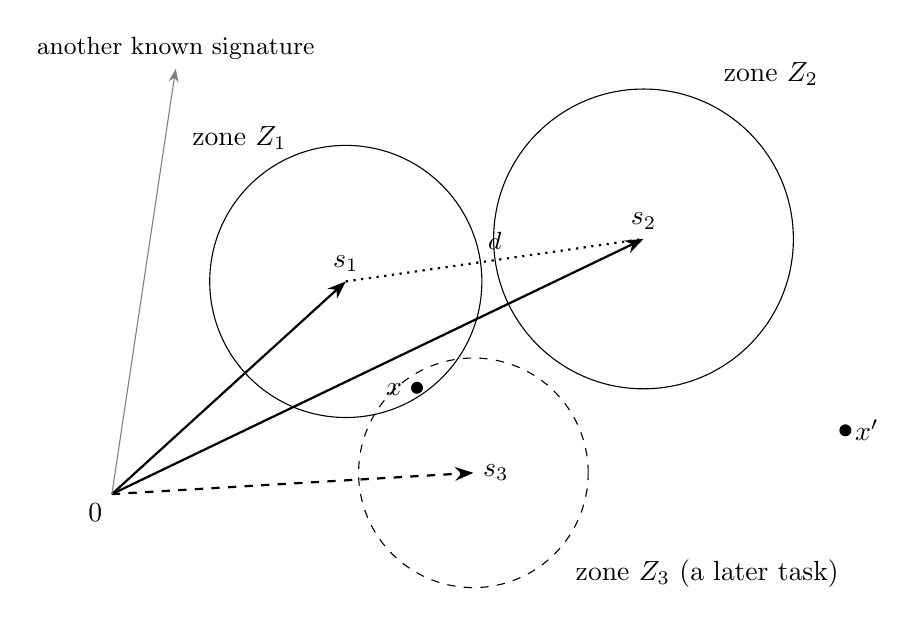
\begin{tikzpicture}[scale=1.35]
\coordinate (O) at (0,0);
\coordinate (s1) at (2.2,2.0); \coordinate (s2) at (5.0,2.4); \coordinate (s3) at (3.4,0.2); \coordinate (b) at (0.6,4.0);
\draw (s1) circle (1.28); \draw (s2) circle (1.41); \draw[dashed] (s3) circle (1.08);
\draw[->, thick] (O)--(s1); \draw[->, thick] (O)--(s2); \draw[->, thick, dashed] (O)--(s3); \draw[->, gray] (O)--(b);
\draw[dotted, thick] (s1)--(s2) node[midway, above]{\small $d$};
\node[above] at (s1) {$s_1$}; \node[above] at (s2) {$s_2$}; \node[right] at (s3) {$s_3$};
\node[above] at (b) {\small another known signature};
\node at (1.2,3.35) {zone $Z_1$}; \node at (6.2,3.95) {zone $Z_2$}; \node at (5.6,-0.75) {zone $Z_3$ (a later task)};
\fill (2.87,1.0) circle (1.6pt); \node[left] at (2.82,0.98) {$x$};
\fill (6.9,0.6) circle (1.6pt) node[right]{$x'$};
\node[below left] at (O) {$0$};
\end{tikzpicture}

{\small Arrows: signatures (vectors). Circles: zones. $d$ is the distance from $s_2$ to its nearest
known signature $s_1$, and $R_2 = d/2$.\\ $x$ is inside a zone. $x'$ is outside every zone.}
\end{center}

\step{8} \textbf{Why half.} Let $j$ be an older task. By Step 6, $R_k \le \tfrac12\|s_k - s_j\|$, so
\[ \|s_j - s_k\| \;\ge\; 2R_k \;>\; R_k \qquad (\text{when } R_k > 0). \]
The older signature $s_j$ is outside the new zone $Z_k$: a new task can never claim the unedited
inputs of an older task.

\subsection*{6.3 The route}

\step{9} If $x$ lies in at least one zone, it is \emph{certified}, and it goes to the \emph{oldest} zone
that contains it. If it lies in no zone, it goes to the nearest zone, without a certificate.
\[ \rho_T(x) = \min\{\,k \le T : x \in Z_k\,\} \quad \text{if } x \text{ is certified.} \]

\begin{center}
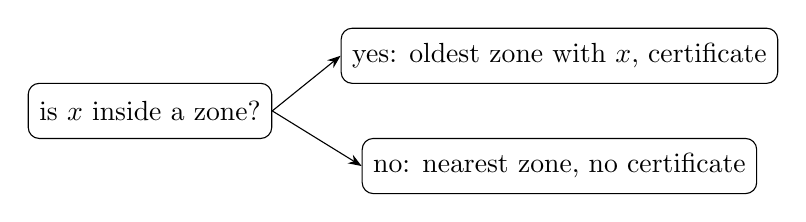
\begin{tikzpicture}
\node[box] (q) at (0,0) {is $x$ inside a zone?};
\node[box] (y) at (5.2,0.7) {yes: oldest zone with $x$, certificate};
\node[box] (n) at (5.2,-0.7) {no: nearest zone, no certificate};
\draw[->] (q.east)--(y.west); \draw[->] (q.east)--(n.west);
\end{tikzpicture}
\end{center}

\subsection*{6.4 Why a certified answer never changes}

Let $x$ be certified at time $T$ with route $j$. Take any later time $T'$.

\step{10} Write the set of zones that contain $x$ at time $T$:
\quad $A_T = \{\,k \le T : x \in Z_k\,\}$, \ and $j = \min A_T$.

\step{11} Zones are never changed or removed. So every zone in $A_T$ still contains $x$ at time $T'$.
New tasks can only add zones with larger numbers:
\[ A_{T'} \;=\; A_T \ \cup\ \{\,k : T < k \le T',\ x \in Z_k\,\}. \]

\step{12} Every number in the second set is larger than $T$, and $j \le T$. So the new numbers are all
larger than $j$, and the smallest number of $A_{T'}$ is still $j$:
\[ \rho_{T'}(x) = \min A_{T'} = \min A_T = j = \rho_T(x). \]

\step{13} The route did not change. By Section 2, the answer did not change:
\[ \boxed{\ x \text{ certified at } T \ \Longrightarrow\ y_{T'}(x) = y_T(x) \ \text{ for every later } T' \text{ and any later tasks}\ } \]

\begin{center}
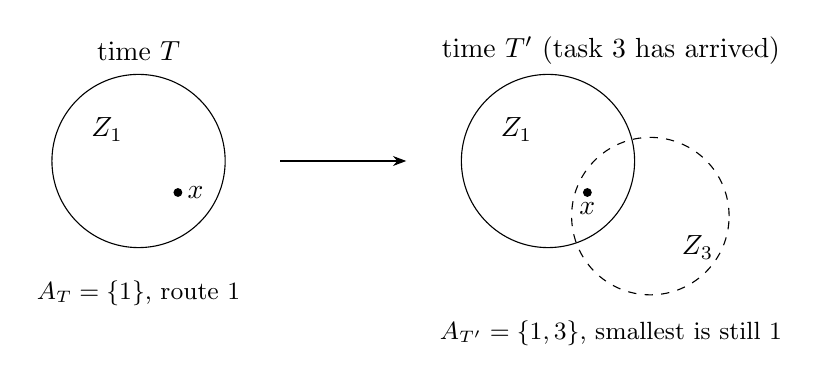
\begin{tikzpicture}
\node at (1.4,2.0) {time $T$}; \draw (1.4,0.6) circle (1.1); \fill (1.9,0.2) circle (1.6pt) node[right]{$x$}; \node at (1.0,1.0) {$Z_1$};
\node at (7.4,2.0) {time $T'$ (task 3 has arrived)}; \draw (6.6,0.6) circle (1.1); \draw[dashed] (7.9,-0.1) circle (1.0); \fill (7.1,0.2) circle (1.6pt) node[below]{$x$}; \node at (6.2,1.0) {$Z_1$}; \node at (8.5,-0.5) {$Z_3$};
\draw[->] (3.2,0.6)--(4.8,0.6);
\node[below] at (1.4,-0.8) {\small $A_T=\{1\}$, route 1};
\node[below] at (7.4,-1.3) {\small $A_{T'}=\{1,3\}$, smallest is still 1};
\end{tikzpicture}
\end{center}

$x$ now also lies in the later zone $Z_3$, but the oldest zone wins: \emph{finders keepers}.

%=====================================================================
\section*{7. In one line each}

\begin{tabular}{@{}ll@{}}
FinderLoRA & score every task with $V_T$, go to the largest; no instruction needed.\\
Audit & share of held-out inputs whose route changed $=$ estimate of changed answers.\\
KeeperLoRA & a newcomer takes $x$ only above a threshold; change $\le (T_{\text{end}}-j)(\nu+1)/(m+1)$.\\
ClaimLoRA & oldest zone wins; inside a zone the answer never changes.\\
\end{tabular}

\end{document}
